\section{Volle Synchronisation einer Simulation}
Das Ziel ist, auf zwei Maschinen (oder Prozessen) jeweils eine Simulation zu haben, welche miteinander in Echtzeit synchronisiert werden.\\
Zu diesem Zweck wird eine Synchronisation zunächst mit einer Master-Slave-Strategie umgesetzt. Eine Maschine dient dabei als Server, eine als Client.
Der Server hat die Aufgabe, den Status der Simulation auf eine neue Simulationszeit fortschreiten zu lassen. Ein solcher Simulationsschritt wird Tick genannt (vgl. im Anhang den Abschnitt \ref{sec:tick}). Die Instanz der Simulation auf dem Server ist immer vollständig, d.h.~sämtliche Simulationsinhalte sind auf dem Server immer präsent. Ein lokaler Benutzer kann sich an der Servermaschine direkt zur Simulation verbinden und hat sämtliche benötigten Informationen sofort parat.\\
Ein Client dagegen ist meist nicht vollständig. Der Client hat die Aufgabe, vom Server gesendete Aktualisierungen für Simulationsinhalte anzunehmen und zu verarbeiten. Der Client hat unter Umständen nur die für ihn relevanten Simulationsinhalte lokal vorhanden. Der Client führt keine Ticks, d.h.~keine Simulation selbstständig durch. Der Client hat die Möglichkeit, in Verbindung mit einem eigenen lokalen Benutzer eine grafische Ausgabe anhand der ihm bekannten Simulationsinhalte zu generieren und über einen Kontrollstatus Eingaben an eine Remote-Simulation zu liefern. 

\subsection{Client-Eingaben}
Dem Client ist es unter Master-Slave-Architektur nicht erlaubt, irgendwelche Simulationsinhalte direkt zu schreiben. Ein Benutzer soll also nicht einmal seine eigene Figur (Userentität) im simulierten Raum selbst bewegen.\\
Es scheint praktisch, die in der Fernsteuerung umgesetzten Eingabemethoden wiederzuverwenden. Die Methode ist bereits optimiert in Aspekten der Bandbreite, die zu übertragene Information ist bereits auf essentielle Use-Cases für die Steuerung einer Figur reduziert. Die Semantik des Kontrollstatus als Bedienerintention scheint richtig: Der Client hat als Slave keine kontrollierenden Rechte gegenüber Inhalte der Simulation und kann über den Kontrollstatus nur Vorschläge liefern, welche die Simulation auf dem Server zu ihrer Diskretion interpretieren kann.

\subsection{Zeitsynchronisation}

Ein Ziel der Synchronisation der Simulation auf verschiedenen Rechenmaschinen ist die Illusion von Gleichzeitigkeit, trotz der von der Latenz verursachter Seiteneffekte, zu erzeugen.
Bei Synchronisationsvorgängen von gezeiteten Simulationsinhalten ist eine gemeinsame Zeitbasis sinnvoll.
Auf verschiedenen Rechenmaschinen liegen jedoch unterschiedliche Uhren vor, welche sich in durch den Einfluss der Hardware oder des Betriebssystems in Epoche und Clockrate unterscheiden können. Typische Symptome sind Drift und Jitter bei Uhren auf verschiedenen Systemen.
Eine Synchronisation der Zeitbasen selbst bedeutet regelmäßig die Uhren zu stellen und die Umrechnung unterschiedlicher Uhrenarten oder Zeitformaten bereitzustellen.\\
Zunächst wird eine minimale Genauigkeit der Zeitabtastung in Mikrosekunden auf allen verwendeten Maschinen versichert . Zudem gilt die Unterscheidung der messbare Zeitbasen einer Realzeit und der relativ dazu laufenden Simulationszeit (vgl. Appendix \ref{sec:time}).\\
Aus der o.g. Master-Slave-Strategie folgt, dass der Server (Master) die Simulationszeit vorgibt, d.h.~es ist die Aufgabe der Clients, ihre Simulationszeituhren einzustellen. 
Bei der Zeitsynchronisation mit dem Server wird die Latenz der Realzeit beidseitig gemessen.
Dies muss hier in beiden Richtungen geschehen, da die einzelnen Signallaufzeiten ohne vorher synchrone Uhren nicht auf der selben Realzeitbasis existieren und Zeiten sonst nicht vergleichbar ermittelt werden können. 
Die einzelne Signallaufzeit kann abgeschätzt werden, indem die 2-Wege-Laufzeit halbiert wird. Dazu werden zu jedem UDP-Paket, welche eine frequente Kommunikation umsetzen, zwei Zeitstempel versendet, wobei einer die aktuelle Serverzeit und der andere die aktuelle Clientzeit beinhaltet.
So legt ein Zeitstempel jeweils Hin- und Rückrichtung zurück und die Zwei-Wege-Laufzeit kann anhand der Stempel in empfangenen Paketen an beiden Knoten ermittelt werden.\\
Prinzipiell ist zum alleinigen Zweck der Synchronisation der Simulation auch nur die Synchronisation der Simulationszeituhren vonnöten.

\begin{figure}
    \centering
    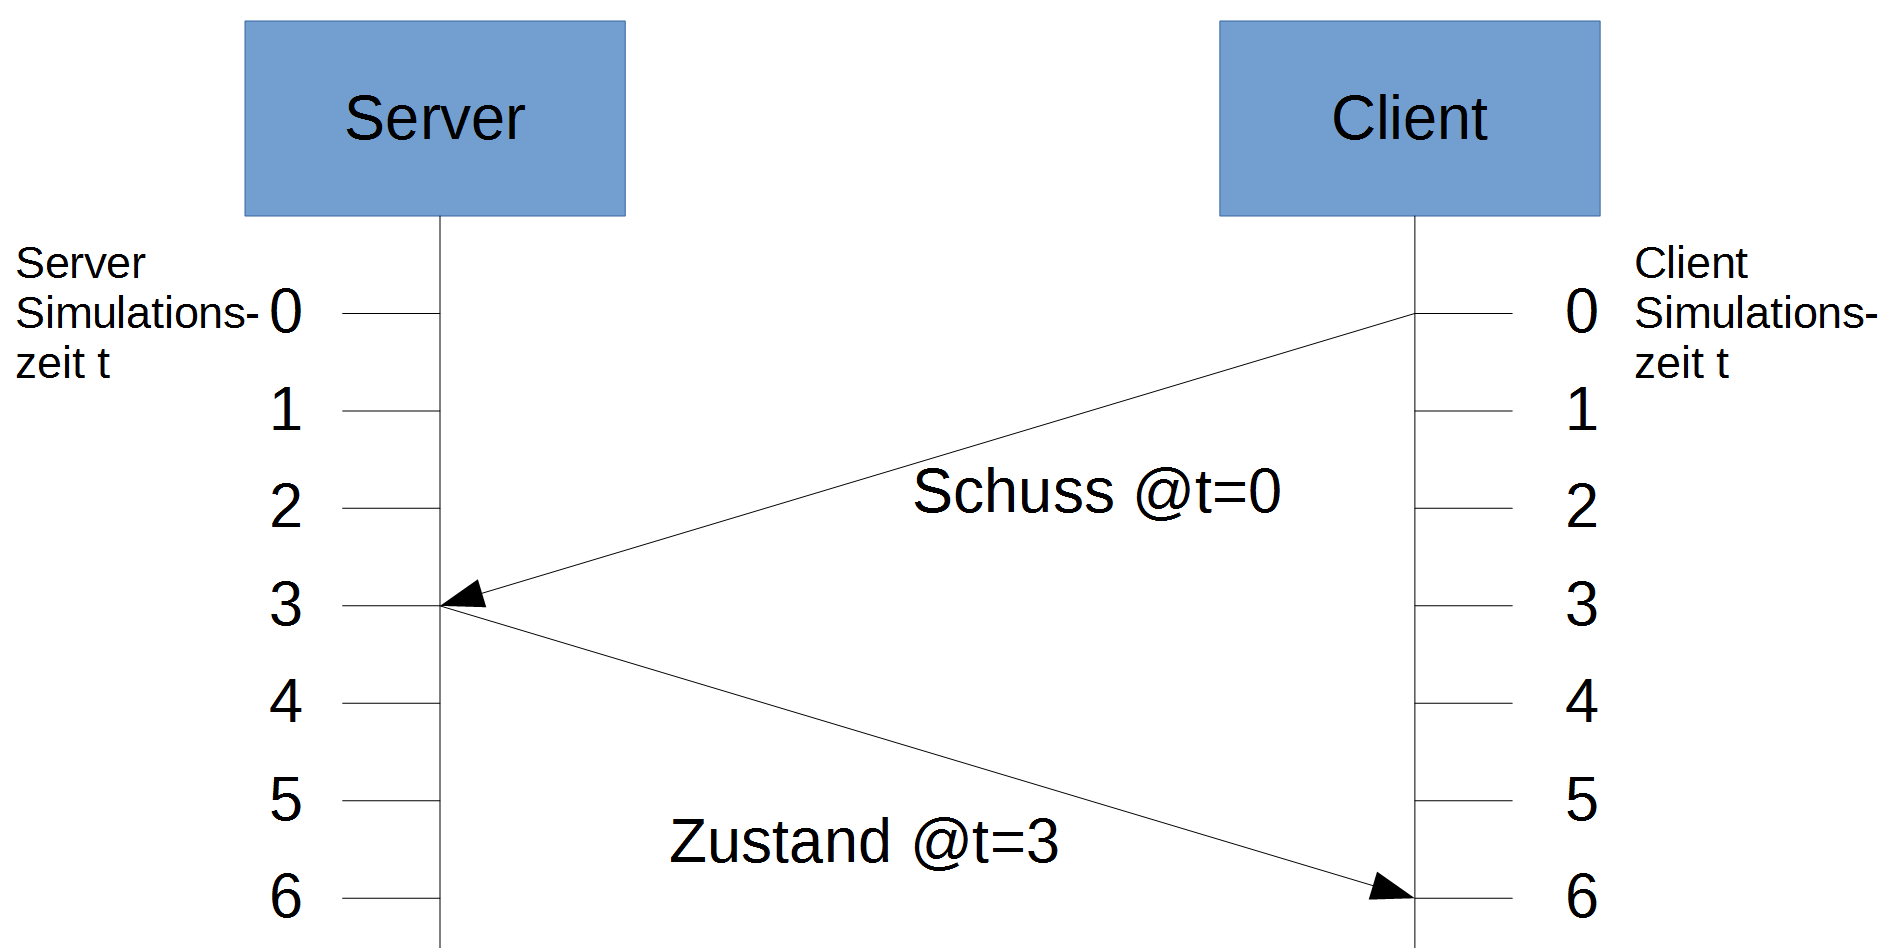
\includegraphics[width=0.75\textwidth]{./Zeichnung1a.png}
    \caption{Diagramm über Beispielsituation für Uhren, die gleichzeitig eingestellt sind. Gleiche Höhe entspricht Gleichzeitigkeit der echten Zeit. Dargestellt sind außerdem Beispielpakete mit Inhalt und Absendezeitpunkt in Simulationszeit.}
    \label{fig:zeichnung1a}
\end{figure}

Die offensichtlichste Variante der Einstellung der Simulationszeituhr am Client ist, möglichst Gleichzeitigkeit mit der Serveruhr anzustreben. Diese hätte allerdings Implikationen für die Implementierung, wie in Abb.~\ref{fig:zeichnung1a} ersichtlich. 
Aktionen, die vom Client ausgelöst werden, kommen erst verspätet am Server an.
Dieser müsste die so erhaltene Information retroaktiv anwenden, um die Richtigkeit aus der Sicht des Clients herzustellen.
Dann muss im schlimmsten Fall die gesamte Simulation wiederholt werden (von 0 bis~3), um einen korrekten Zustand zu Zeitpunkt~3 herzustellen. Dies benötigt Speicher, für die Speicherung alter Simulationszustände, und Rechenleistung zur wiederholten Neuberechnung von schon behandelten Simulationszeitpunkten. Den zweiten Teil der Arbeit hat der Client. Er erhält die Simulation zum Zeitpunkt~3 und muss daraus ein Bild für den Benutzer generieren, das den Zeitpunkt~6 darstellt. Dies kann auf 2 Arten erreicht werden.
\begin{enumerate}
\item Simulation am Client für die fehlenden Zeitschritte simulieren und das Ergebnis anzeigen. Dies hat den Vorteil, dass die Anzeige am Bildschirm am genauesten den echten Zustand darstellt, da alle Informationen in das Bild einfließen. Nachteile sind:
\begin{itemize}
 \item ein höherer Berechnungsaufwand, da die Simulation nun nicht nur am Server, sondern auch am Client stattfinden muss. 
 \item Der Server muss nicht nur Informationen, die die Anzeige am Bildschirm betreffen, versenden, sondern auch Werte, die nur für den Simulationsschritt wichtig sind.
 \item Wenn am Server etwas passiert, von dem der Client noch keine Informationen hat (z.B. Aktion eines anderen Spielers, die noch nicht angekommen ist), ist der Zustand der Simulation am Client nicht mehr valide. Der Client müsste dann also entweder alte Simulationszustände speichern und eine Neuberechnung durchführen, oder er ließe sich vom Server die komplette Simulation erneut zusenden.
\end{itemize}
\item Der Client rechnet die Anzeige auf unverbindliche Art und Weise nach vorne. Es wird hierbei dieselbe Extrapolation verwendet, die das Grafikmodul verwenden kann, um zwischen wenigen Simulationsschritten viele Bilder am Bildschirm zu erzeugen. Dazu werden vereinfachte Annahmen getroffen, wie z.B.~ dass Objekte sich linear bewegen, anhand der letzten bestätigten Position und letzten bestätigten Geschwindigkeit. Die resultierende Anzeigeposition wird nicht gespeichert, sondern nur zur momentanen Anzeige verwendet.
Vorteile sind die einfachere Berechnung und geringere benötigte Bandbreite vom Server. Außerdem hängt die benötigte Rechenzeit nicht davon ab, wie weit der letzte bestätigte Zeitpunkt zurückliegt. 
Nachteilig ist die geringere Genauigkeit der Anzeige gegenüber dem eigentlich korrekten Simulationszustand. Es werden auf dem Client so keine Interaktionen, wie z.B.~das Treffen eines Projektils, berücksichtigt. 
In der Praxis ist dies in den meisten Fällen aber nicht sehr kritisch, da innerhalb von Bruchteilen einer Sekunde der Server den Simulationszustand mit enthaltenen Auswirkungen von Interaktionen aktualisiert. Die grafische Diskrepanz zum Simulationszustand tritt also am Client nur für sehr kurze Zeit auf.\\
\end{enumerate}
\begin{figure}
    \centering
    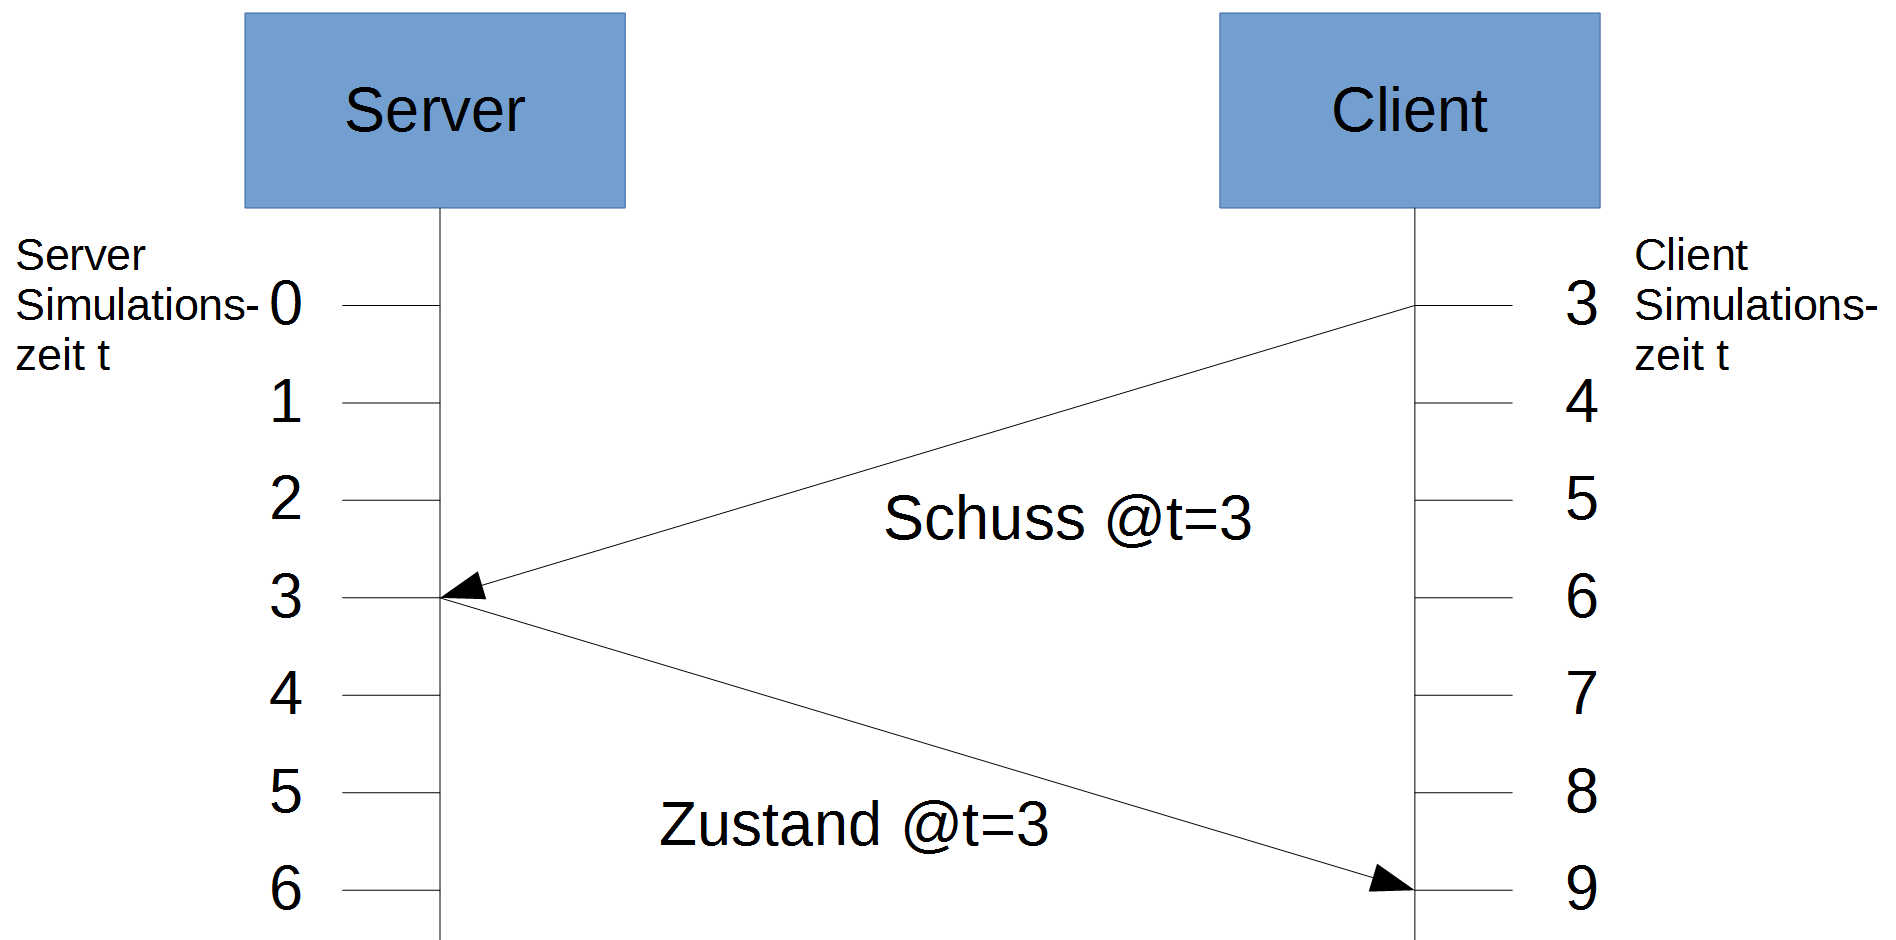
\includegraphics[width=0.75\textwidth]{./Zeichnung2a.png}
    \caption{Diagramm über Beispielsituation für Simulationszeit-Uhren, die zeitversetzt so eingestellt sind, dass der Client um die Latenz Client-zu-Server vorwärts zeitversetzt ist. Gleiche Höhe entspricht Gleichzeitigkeit der echten Zeit. Dargestellt sind außerdem Beispielpakete mit Inhalt und Absendezeitpunkt in Simulationszeit.}
    \label{fig:zeichnung2a}
\end{figure}
Eine weitere Möglichkeit, Uhren am Client einzustellen, ist die Uhr um die Einweg-Latenzzeit zum Server in die Zukunft zu stellen (siehe Abb.~\ref{fig:zeichnung2a}). In diesem Fall kann der Server die Aktionen vom Client als gegenwärtig betrachten und es müssen so keine retroaktiven Berechnungen durchgeführt werden.\\
Als Beispiel in der Abbildung dient der Schuss eines Projektils.
Der Schuss zum Zeitpunkt~3 des Clients ist also zu Zeitpunkt~3 am Server vorhanden, sodass er diesen wie eine lokale Eingabe in der Gegenwart verarbeiten kann. Speicherung alter Zustände oder wiederholtes Berechnen des selben Zeitpunktes sind nicht mehr nötig.
Aus diesen Gründen wurde dieses Modell gewählt. Der Server behandelt alle eingehenden Pakete mit Aktionen vom Client als in der Gegenwart auftretend.

Für den Client ändert sich gegenüber dem anderen Ansatz lediglich die Größe der Zeitdifferenz, die mit beiden o.g. Methoden zu einem aktuellen Bild führt. Für dieses Projekt wurde diejenige gewählt, die rein grafisch extrapoliert. Die grafische Diskrepanz zum Simulationszustand, obwohl nun u.U.~größer, wird immer noch als marginal eingeschätzt.\\

Die Berechnung von zeitverschobenen Ereignissen wird so nahezu komplett dem Client überlassen.
Das führt zudem zu einer hocherwünschten Robustheit des Simulationszustandes am Server gegenüber der Latenz, vor allem im Bezug auf hohe Latenzen zu einzelnen Clients. Die Simulation am Server ist auf diese Weise stabil, während die Seiteneffekte von hoher Latenz gerechterweise nur diejenigen Clienten betreffen, welche eine hohe Latenz zum Server haben.
Bei retroaktiven Strategien würden alle Clienten unter der hohen Latenz eines einzigen leiden, da dessen extrem verspätete Information so auf alle Clienten retroaktiv verteilt werden müsste.

%%TODO discussion : Mehrere spieler ? Latenztoleranz? Maximale vorausberechnung von Clients sonst drop? Ja, alles weitere Probleme aber wäre zuviel blah da das sowieso nicht das gewählte Modell ist.

\begin{figure}
    \centering
    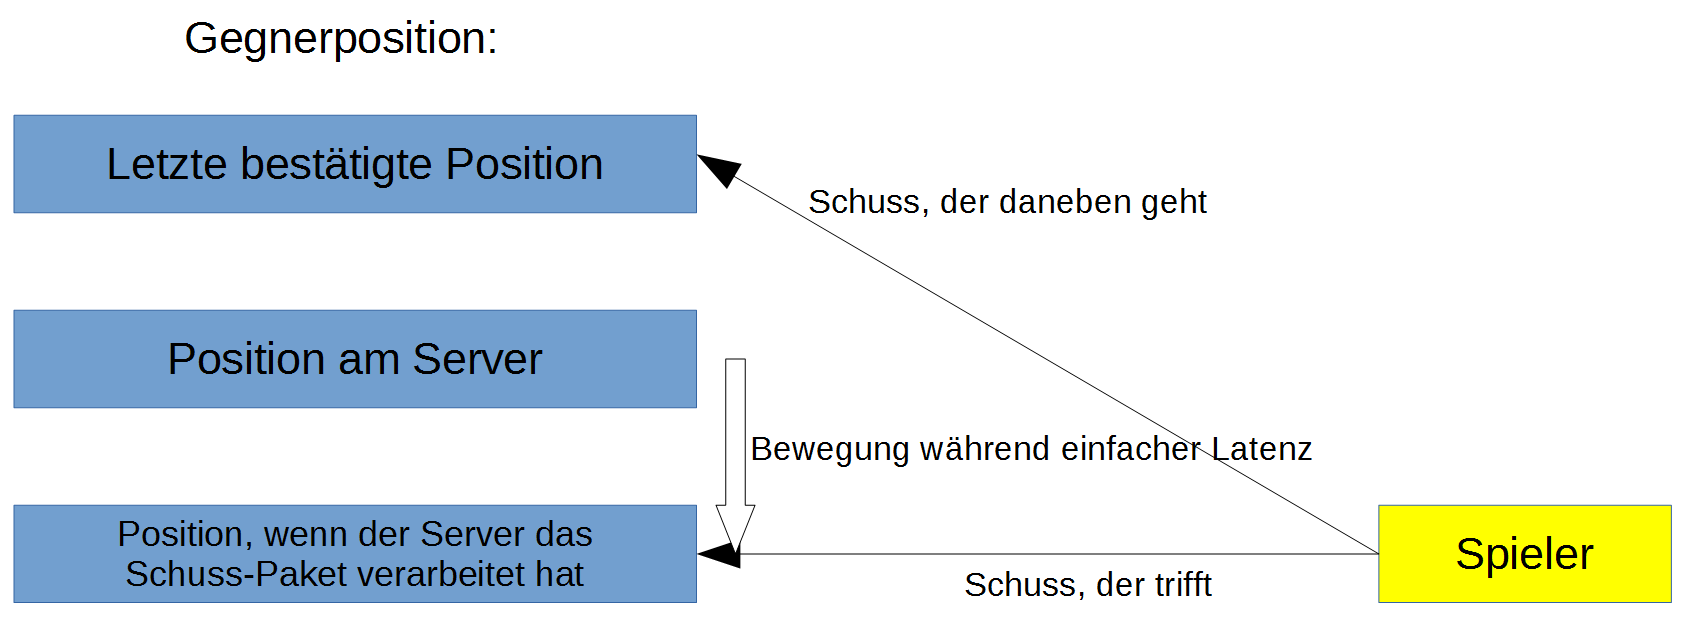
\includegraphics[width=0.85\textwidth]{./Gegnerposition1a.png}
    \caption{Diagramm über eine Beispielsituation, in der ein Spieler auf einen Gegner schießt. Der Ort im Diagramm entspricht größtenteils Maßstabsgetreu der Position in der Simulation (für Gegner, Spieler und Schüsse). Die einfachen Pfeile stellen Schüsse des Spielers dar.}
    \label{fig:gegnerposition1a}
\end{figure}

Der Grund, dass die Extrapolation überhaupt notwendig ist, zeigt Abb.~\ref{fig:gegnerposition1a}. Die Berechnungslatenz und die Paketlatenz werden in der Implementierung (und in den Abbildungen) nur gemeinsam, als Gesamtlatenz verwendet. Zu sehen ist, dass wenn der Spieler auf die letzte bestätigte Position schießt, der Gegner sich zu einer neuen Position bewegt hat, bis die Informationen über den Schuss am Server ankommen. Der Schuss würde verfehlen. Die Aufgabe der grafischen Extrapolation ist es also, den Gegner an dem Ort anzuzeigen, wo er wahrscheinlich sein wird, wenn die Informationen über den aktuellen Client-Zustand in der Server-Simulation ankommen. Der Spieler kann dann wie lokal gewohnt auf bewegliche Ziele schießen, ohne die Latenz zum Server miteinbeziehen zu müssen.
Die Latenz, die für eine korrekte Extrapolation eingerechnet werden muss, muss die Zwei-Wege-Gesamtlatenz inklusive Berechnungslatenz auf Client und Server sein.\\

%%TODO TODO resolved?
Um die Daten für die oben beschriebene Extrapolation möglichst genau zu ermitteln, bietet es sich an, die benötigten Daten an die normalerweise anfallende Kommunikation anzuhängen, die mit exakt der dafür korrekten Latenz arbeitet. Die Uhr des Servers wird als normales Datenelement (Syncable, später in Abschnitt~\ref{sec:syncable} beschrieben) an die Clients übertragen. Sie beinhaltet die aktuelle und gewünschte Simulationszeitrate relativ zur Realzeit (z.B. 0,1 bedeutet 10-fache Zeitlupe), und den aktuellen Zeitpunkt am Server. 
Client und Server versenden im Zuge der Latenzberechnung in jedem UDP-Packet ihre aktuellsten Realzeitstempel. Damit kann der Server den aktuellsten bekannten Zeitpunkt der Uhr für jeden Client mitführen. 
Dieser Zeitpunkt wird in jedem UDP-Packet, welches die Simulationsuhr auf dem Client aktualisiert, mitgeführt werden.
Wenn der Client nun ein Update der Uhr erhält kann er daraus die Zuordnung Realzeitzeitpunkt der Clientuhr zu Simulationszeitpunkt der Serveruhr (unter Berücksichtigung der Zeitrate) berechnen und so die Uhrensynchronisation beider Simulationszeituhren zwischen Client und Server herstellen. Ein Beispiel für das Verfahren ist in Abb.~\ref{fig:zeichnung3a} zu sehen.
\begin{figure}
    \centering
    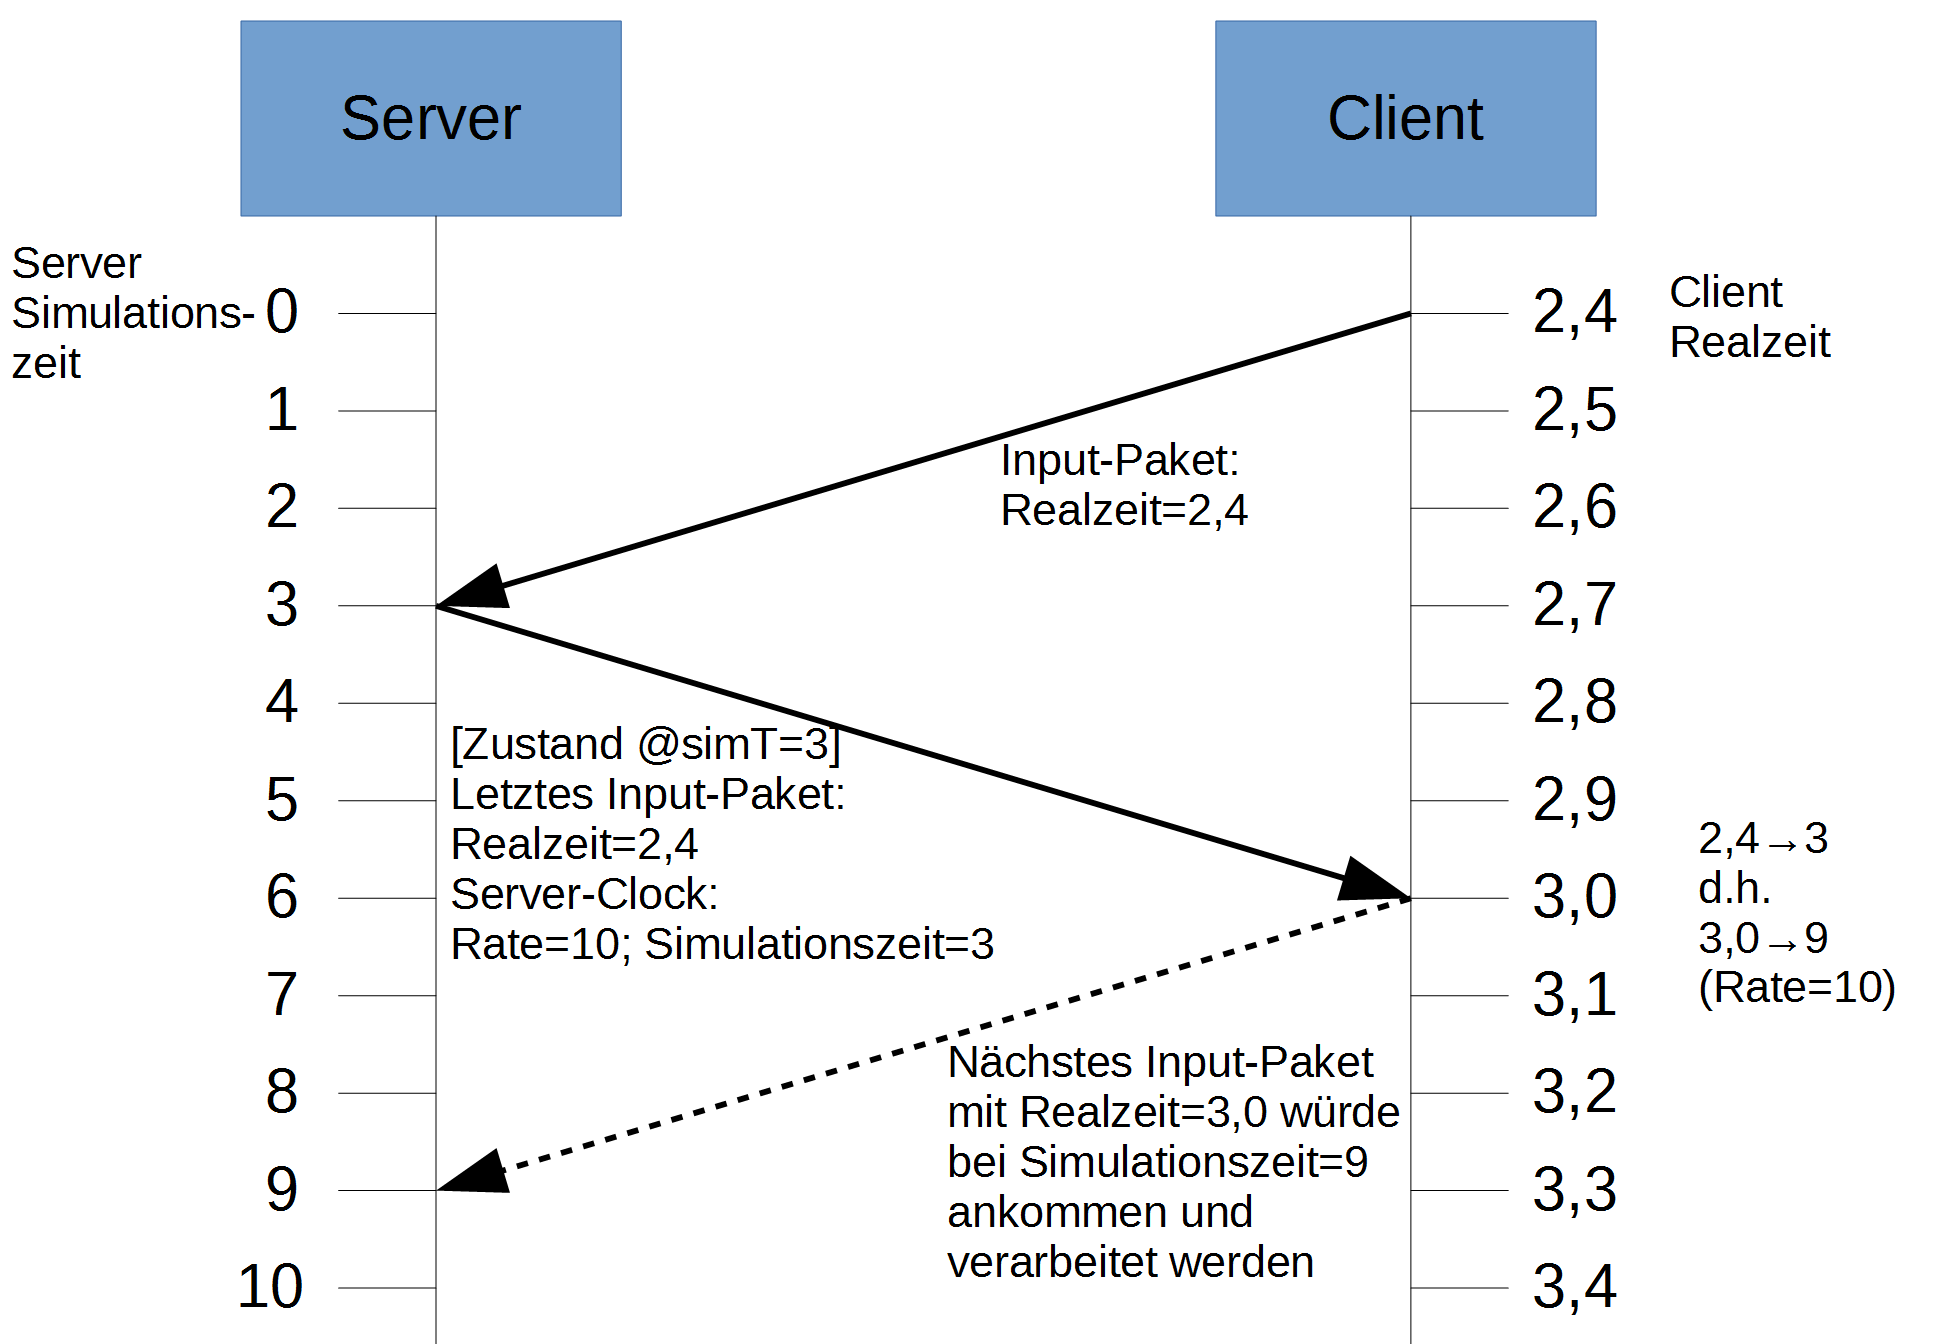
\includegraphics[width=0.75\textwidth]{./Zeichnung3a.png}
    \caption{Diagramm über Beispielsituation bei Simulationszeit-Uhrensynchronisation, mit zeitversetzten Uhren wie in Abb.~\ref{fig:zeichnung2a}. 
Gleiche Höhe entspricht Gleichzeitigkeit der physikalisch echten Zeit 
(nicht der Zeit, welche die jeweiligen Maschinen messen und als Realzeit interpretieren). Der Client errechnet aus den Daten in den Synchronisierungspaketen diejenige Simulationszeit, die dem Eintreffen am Server und der Verarbeitungszeit eines hypothetischen Pakets entspricht, wenn es sofort abgesendet werden würde.}
    \label{fig:zeichnung3a}
\end{figure}


\subsection{Übertragung der Simulationsinhalte zum Client}
\label{sec:syncable}
Um die Simulationsinhalte übertragen zu können, wurde zunächst ein Interface entworfen, über das die Daten gelesen und geschrieben werden können. Das Interface wird hier Syncable genannt.
Zunächst müssen die möglichen Datensätze in Kategorien unterteilt werden:
\begin{itemize}
\item Update-Daten: Daten, die ein bestehendes Objekt in den neuen, aktuellen Zustand überführen (z.B. Position). Es handelt sich hierbei immer um Statusinformation.
\item Vollständiger Datensatz: Daten, die übertragen werden müssen, um ein neues Objekt zu erstellen. Diese Daten beinhalten meist alle Update-Daten und beinhalten zusätzlich noch die Daten, die einmalig zur Initialisierung notwendig sind (z.B. Größe eines konkreten Gegners).
\end{itemize}
Ein konkretes Syncable definiert Serialisierungs- und Deserialisierungsmethoden für beide Kategorien von zu Datenpaketen statt. Für Pakete wird die Programmbibliothek SFML (siehe Quelle~\cite{sfml}), genauer deren Netzwerkkomponente, verwendet, welche eine plattformunabhängige Implementierung eines Datenpaket mitbringt, z.B. im Kontext Endianess.\\
Serialisierte Informationen mehrerer Syncables werden in Paketen gesammelt.
Bei der Deserialisierung passiert der umgekehrte Prozess der Serialisierung: Die Daten werden aus dem Paket entnommen und jede konkrete Instanz eines Syncables führt entsprechend dieser ein Update durch.\\
Bei der Deserialisierung vollständiger Daten handelt es sich um die Übertragung der Existenz eines auf der empfangenden Maschine unbekannten Syncables, d.h.~die adressierte Syncable-Instanz existiert beim Erhalt der vollständigen Information noch nicht, weshalb für diesen Fall ein Konstruktionsmechanismus bereitgestellt wird, welcher aus den gelieferten Informationen ein konkretes Objekt erstellen kann.\\
Um den erwünschten Typen des neuen Objekts zu ermitteln wird eine Typidentifikationsnummer für den Zweck der Objekterstellung mitübertragen.
Der Empfänger kreiert weiter die erwünschten Objekte mittels eines Factory-Patterns.\\
Im Rahmen des Projektes wurden also alle bestehenden Simulationsbestandteile, die übertragen werden müssen, zu Syncables. Für jedes davon wurden jeweils nur diejenigen Daten selektiert, die für die grafische Anzeige am Client relevant sind.\\

Instanzen von Syncables werden zentral pro Maschine in einem sog.~Syncable-Manager, verwaltet. 
Dieser wird initial mit seinem ersten Syncable bestückt: der Simulation selbst, welche das Interface ebenfalls implementiert. Die Simulation enthält die Simulationsinhalte als weitere Syncables. Es wird so implizit eine Baumstruktur erstellt. Der Syncable-Manager verwaltet sämtliche Syncables jedoch nicht in einer Baumstruktur, sonder in einem flachen Container.\\
Eine Simulation bietet weiter dediziert Informationen in Form konsumierbarer Ereignisse über Objektneuerzeugungen oder -löschungen an, auf welche der Syncable-Manager, vor allem am Server, reagiert.\\
Die Ereignisse liefern dabei zur Erzeugung beispielsweise die vollständige Information.\\
Instanzen von Syncables werden am Syncable-Manager über eine eindeutige Identifikationsnummer unterschieden. Diese wird vom Server festgelegt und an Clients entsprechend im Rahmen der Objekterstellungsevents propagiert. Die Nummer kann weiter für alle anderen Zwecke verwendet werden, welche eine Spezifizierung eines Syncables benötigt werden, z.B.~Löschung.\\
Die Ereignisse werden auf Grund der Kritikalität der Einhaltung ihrer Reihenfolge und der Anforderung der Übertragungsversicherung über TCP übertragen.\\
Updates (Teilserialisierungen), die den Zustand eines bestehenden Syncables aktualisieren haben andere Anforderungen: Fehlende Updates sind unkritisch, da sie durch das nächste Update vollständig ersetzt werden. Veraltete Updates, die verspätet ankommen können auf Grund von nicht eingehaltenen Echtzeitanforderungen als nicht aktuell genug verworfen werden. Aus diesen Gründen ist hier UDP die beste Wahl.\\
Bei Events ist die benutzte Bandbreite durch die Anzahl und Größe der Events festgelegt, da sie nicht weggelassen werden können. Bei Updates bedeutet ein fehlendes Paket jedoch nur eine etwas ungenauere Positionsextrapolation, die die Grafikkomponente erzeugt. Die Rate, mit der Updates versendet werden, kann also variabel gewählt werden. Da Netzwerkverbindungen immer eine Bandbreitenlimitierung aufweisen, sollte diese beachtet werden und als Grenze für die Rate der Updates dienen.\\
Die Verfügbare Anzahl an Bytes entsprechend einer eingestellten maximalen Bandbreite stellt die Netzwerkkomponente zu jeder Zeit zur Verfügung.
Der Syncable-Manager ist so konzipiert, dass er beim Füllen von Paketen ein Maximum verfügbarer Bytes berücksichtigt.
Bei Update-Paketen werden solange Updates von einzelnen Syncables eingefügt, bis die Maximalgröße ein weiteres Einfügen verhindert. Die Syncables, die im aktuellen Paket enthalten sind, werden nach dem Round-Robin-Verfahren ausgewählt (maximal 1~Runde pro Update-Paket).\\
Die einzelnen Updates sind durch die eindeutige ID von Syncables am Client adressiert.


\subsection{Besonderheiten}
Die Implementierung weist noch einige Besonderheiten auf:%TODO satz weglassen?
\begin{itemize}
\item Das Terrain wird nicht übertragen, da es mit einem plattformunabhängigen Zufallsgenerator mit festem Seed erzeugt wird und daher auf den verschiedenen Rechnern identische Resultate liefert. Terrain kann sich außerdem nicht verändern. Aus diesen Gründen kann der Client es einfach selbst bei Bedarf erzeugen (und wieder verwerfen, sobald sich der Spieler von einem Ort zu weit entfernt).
\item Die Sichtrichtung einer Spielerfigur, und somit die grafisch angezeigte Perspektive am Client, wird aktuell noch vom Server bestimmt, ohne dass der Client für die Kamera im 3D-Raum eine eigene Schätzung verwendet. 
Ein Spieler muss so beim Drehen seiner Sicht die Zwei-Wege-Latenz zum Server in Kauf nehmen. Zwar handelt der Server nach dem hier gezeigten Synchronisationsschema mit Gleichzeitigkeit, der Unterschied wird jedoch am Client grafisch merkbar, wenn sich die Perspektive schnell ändert während z.B.~geschossen wird. Projektile sind prinzipiell da wo sie sein sollen, das lokal angezeigte Fadenkreuz u.U.~allerdings nicht. Für einen Shooter ist die Flüssigkeit des Bildes  beim Zielen essentiell.
Dies wäre somit die höchste Priorität für Erweiterungen des klassischen linearen Extrapolationsmodells der Grafik am Client, die lokal anliegenden Eingabeereignisse eigenständig mit einzubeziehen. Problematisch bei der Umsezung ist dort, dass der Server bestimmt, wann der Spieler seine Waffe abfeuert. Er bestimmt damit auch den Rückstoß, der die Blickrichtung ändert.
\item Das Löschen von Syncables (auf Befehl des Servers) kann nicht abstrakt erfolgen, da innerhalb der Simulation durch die durch Komposition verursachte implizite Baumstruktur verschiedene Klassen von verschiedenen Komponenten verwaltet werden und die jeweils Korrekte über die Löschanfrage benachrichtigt werden muss. Über die in Abschnitt~\ref{sec:syncable} beschribene Typ-ID ist eine Differenzierung zur Laufzeit möglich.
\item Geräusche, die alle als Reaktion auf ein Ereignis im Spiel auftreten (also vom Server angeordnet werden), wurden im Rahmen des Projekts nicht synchronisiert. Der Grund dafür ist, das aufgrund der Art und Weise, wie diese bisher implementiert sind und eine weitgehende Neuimplementierung des Features notwendig wäre, um auf dem Client zu funktionieren. Das wurde für den Rahmen des Projekts als zu Aufwändig eingeschätzt.
\item Viele Bestandteile der Synchronisierungsimplementierung wurden so entwickelt, dass es prinzipiell möglich ist, den Status Server/Client/lokale Simulation zur Laufzeit zu wechseln. Dies ermöglicht es, weiterzuspielen, wenn der Server offline geht. Dieses Feature ist aktuell noch nicht vollständig entwickelt, aber geplant, sodass die aktuelle Implementierung keine Hürden dafür aufweist.
\item In der im Projekt verwendeten Programmiersprache C++ bedeutet Besitz (Ownership) von Objekten normalerweise, das Recht und die Pflicht zu haben, diese zu löschen. Für die Synchronisierung über das Netzwerk ist dieses einfache Modell nicht ausreichend. Am Server besitzt die Simulation die in ihr enthaltenen Syncables. Prinzipiell erstreckt sich der Besitz allerdings über das Netzwerk hinweg zum Client. Während normalem Betrieb hat der Server das alleinige Recht, die Löschung von Objekten am Client zu beauftragen. Es gibt jedoch Fälle, wo der Client lokal die Kontrolle übernehmen muss:
\begin{itemize}
\item Beenden des Programms
\item Beenden der Verbindung
\item Verbindung unterbrochen: Client muss sich neu verbinden oder beenden, was beides Löschung aller Objekte bedeutet.
\item Zukünftig auch: Änderung des Status von Client zu lokaler Simulation oder zu Server. Die lokale Simulation hat dann alle Rechte an Syncables, der Syncable-Manager nimmt dann die Slave-Rolle ein.
\end{itemize}
\item Es fand keine signifikante Optimierung der genutzten Bandbreite statt. Das Design ist zunächst sehr allgemein gehalten, um möglichst viele Arten von Simulationsinhalten unkompliziert synchronieren zu können. 
\end{itemize}



